\documentclass[spec, och, labwork]{shiza}
% параметр - тип обучения - одно из значений:
%    spec     - специальность
%    bachelor - бакалавриат (по умолчанию)
%    master   - магистратура
% параметр - форма обучения - одно из значений:
%    och   - очное (по умолчанию)
%    zaoch - заочное
% параметр - тип работы - одно из значений:
%    referat    - реферат
%    coursework - курсовая работа (по умолчанию)
%    diploma    - дипломная работа
%    pract      - отчет по практике
% параметр - включение шрифта
%    times    - включение шрифта Times New Roman (если установлен)
%               по умолчанию выключен
\usepackage{subfigure}
\usepackage{tikz,pgfplots}
\pgfplotsset{compat=1.5}
\usepackage{float}

%\usepackage{titlesec}
\setcounter{secnumdepth}{4}
%\titleformat{\paragraph}
%{\normalfont\normalsize}{\theparagraph}{1em}{}
%\titlespacing*{\paragraph}
%{35.5pt}{3.25ex plus 1ex minus .2ex}{1.5ex plus .2ex}

\titleformat{\paragraph}[block]
{\hspace{1.25cm}\normalfont}
{\theparagraph}{1ex}{}
\titlespacing{\paragraph}
{0cm}{2ex plus 1ex minus .2ex}{.4ex plus.2ex}

% --------------------------------------------------------------------------%


\usepackage[T2A]{fontenc}
\usepackage[utf8]{inputenc}
\usepackage{graphicx}
\graphicspath{ {./images/} }
\usepackage{tempora}

\usepackage[sort,compress]{cite}
\usepackage{amsmath}
\usepackage{amssymb}
\usepackage{amsthm}
\usepackage{fancyvrb}
\usepackage{listings}
\usepackage{listingsutf8}
\usepackage{longtable}
\usepackage{array}
\usepackage[english,russian]{babel}

% \usepackage[colorlinks=true]{hyperref}
\usepackage{url}

\usepackage{underscore}
\usepackage{setspace}
\usepackage{indentfirst} 
\usepackage{mathtools}
\usepackage{amsfonts}
\usepackage{enumitem}
\usepackage{tikz}
\usepackage{minted}

\newcommand{\eqdef}{\stackrel {\rm def}{=}}
\newcommand{\specialcell}[2][c]{%
\begin{tabular}[#1]{@{}c@{}}#2\end{tabular}}

\renewcommand\theFancyVerbLine{\small\arabic{FancyVerbLine}}

\newtheorem{lem}{Лемма}

\begin{document}

% Кафедра (в родительном падеже)
\chair{}

% Тема работы
\title{Отношение эквивалентности и отношение порядка}

% Курс
\course{3}

% Группа
\group{331}

% Факультет (в родительном падеже) (по умолчанию "факультета КНиИТ")
\department{факультета КНиИТ}

% Специальность/направление код - наименование
%\napravlenie{09.03.04 "--- Программная инженерия}
%\napravlenie{010500 "--- Математическое обеспечение и администрирование информационных систем}
%\napravlenie{230100 "--- Информатика и вычислительная техника}
%\napravlenie{231000 "--- Программная инженерия}
\napravlenie{100501 "--- Компьютерная безопасность}

% Для студентки. Для работы студента следующая команда не нужна.
% \studenttitle{Студентки}

% Фамилия, имя, отчество в родительном падеже
\author{Окунькова Сергея Викторовича}

% Заведующий кафедрой
% \chtitle{} % степень, звание
% \chname{}

%Научный руководитель (для реферата преподаватель проверяющий работу)
\satitle{аспирант} %должность, степень, звание
\saname{В. Н. Кутин}

% Руководитель практики от организации (только для практики,
% для остальных типов работ не используется)
% \patitle{к.ф.-м.н.}
% \paname{С.~В.~Миронов}

% Семестр (только для практики, для остальных
% типов работ не используется)
%\term{8}

% Наименование практики (только для практики, для остальных
% типов работ не используется)
%\practtype{преддипломная}

% Продолжительность практики (количество недель) (только для практики,
% для остальных типов работ не используется)
%\duration{4}

% Даты начала и окончания практики (только для практики, для остальных
% типов работ не используется)
%\practStart{30.04.2019}
%\practFinish{27.05.2019}

% Год выполнения отчета
\date{2022}

\maketitle

% Включение нумерации рисунков, формул и таблиц по разделам
% (по умолчанию - нумерация сквозная)
% (допускается оба вида нумерации)
% \secNumbering

%-------------------------------------------------------------------------------------------
\tableofcontents

\section{Постановка задачи}

Цель работы:

Изучение основных свойств бинарных отношений и операций замыкания бинарных отношений.

Порядок выполнения работы:
    \begin{enumerate}
        \item Разобрать определения отношения эквивалентности, фактор-множества. Разработать алгоритмы построения 
        эквивалентного замыкания бинарного отношения и системы представителей фактор-множества.
        \item Разобрать определения отношения порядка и диаграммы Хассе. Разработать алгоритмы вычисления минимальных 
        (максимальных) и наименьших (наибольших) элементов  и построения диаграммы Хассе.
        \item Разобрать определения контекста и концепта. Разработать алгоритм вычисления решетки концептов.
    \end{enumerate}

\section{Теоретические сведения по рассмотренным темам с их обоснованием}

    \subsection{Определение отношения эквивалентности и фактор-множества}

        Бинарное отношение $\varepsilon$ на множестве $A$ называется отношением эквивалентности (или просто эквивалентностью), если оно рефлексивно, симметрично и транзитивно.

        Для любого подмножества $X \subset A$ множество $\rho(X) = \{b \in B: (x, b) \in \rho \text{ для некоторого } x \in X\}$ называется образом множества $X$ относительно отношения $\rho$.

        Образ одноэлементного множества $X = \{a\}$ относительно отношения $\rho$ обозначается символом $\rho(a)$ и называется также образом элемента $a$ или \textbf{срезом} отношения $\rho$ через элемент $a$. 

        Срезы $\varepsilon(a)$ называются классами эквивалентности по отношению $\varepsilon$ и сокращенно обозначаются символом $[a]$. Множество всех таких классов эквивалентности $\{[a]: a \in A\}$ называется фактор-множеством множества $A$ по эквивалентности $\varepsilon$ и обозначается символом $A/\varepsilon$.

        \textbf{Лемма 1.} О замыканиях бинарных отношений.

        На множестве $P(A^2)$ всех бинарных отношений между элементами множества $A$ следующие отображения являются
        операторами замыканий:

        \begin{enumerate}
            \item $f_r(\rho) = \rho \cup \triangle_A$ - наименьшее рефлексивное бинарное отношение, содержащее отношение
            $\rho \subset A^2$,
            \item $f_s(\rho) = \rho \cup \rho^{-1}$ - наименьшее симметричное бинарное отношение, содержащее отношение
            $\rho \subset A^2$,
            \item $f_t(\rho) = \bigcup^\infty_{n=1} \rho^{n}$ - наименьшее транзитивное бинарное отношение, содержащее
            отношение $\rho \subset A^2$,
            \item $f_{eq}(\rho) = f_t f_s f_r(\rho)$ - наименьшее отношение эквивалентности, на содержащее отношение
            $\rho \subset A^2$.
        \end{enumerate}        

    \subsection{Определение отношения порядка}

        Бинарное отношение $\omega$ на множестве $A$ называется отношением порядка (или просто порядком), если оно
        рефлексивно, антисимметрично и транзитивно.

        Порядок $\leq$ на множестве A называется:

        \begin{enumerate}
        \item линейным, если любые два элемента этого множества
        сравнимы, т.е. выполняется $(\forall a, b \in A) (a \leq b \vee b \leq a)$;

        \item полным, если его любое непустое подмножество имеет
        точную верхнюю и точную нижнюю грани;

        \item решеточным, если для любых $\forall a, b \in A$ существуют sup{a,b} и
        inf{a,b}, которые обозначаются соответственно $a \vee b, a \wedge b$ и
        называются также объединением и пересечением элементов a, b.
        \end{enumerate}

        Множество с заданным на нем линейным порядком называется линейно упорядоченным множеством или цепью.

        Множество с заданным на нем решеточным порядком называется решеточно упорядоченным множеством или решеткой.

        Очевидно, что любая цепь является решеткой, но обратное в общем случае не выполняется. 

        Множество $A$ с заданным на нем отношением порядка $\leq$ называется упорядоченным множеством и обозначается $A
        = (A, \leq)$ или просто $(A, \leq)$.

        Элемент $a$ упорядоченного множества $(A, \leq)$ называется:

        \begin{enumerate}
            \item минимальным, если $(\forall x \in A) \text{ } x \leq a \implies x = a$,
            \item максимальным, если $(\forall x \in A) \text{ } a \leq x \implies x = a$,
            \item наименьшим, если $(\forall x \in A) \text{ } a \leq x$,
            \item наибольшим, если $(\forall x \in A) \text{ } x \leq a$.
        \end{enumerate}

        \textbf{Лемма 2.} Для любого конечного упорядоченного множества
        A = (A, $\leq$) справедливы следующие утверждения:

        \begin{enumerate}

        \item любой элемент множества A содержится в некотором  максимальном элементе и содержит некоторый
        минимальный элемент;
        \item если упорядоченное множество A имеет один максимальный (соответственно, минимальный) элемент, то
        он является наибольшим (соответственно, наименьшим) элементом этого множества. 

        \end{enumerate}


    \subsection{Определение диаграммы Хассе}

        Упорядоченное множество $A = (A, \leq)$ наглядно представляется диаграммой Хассе, которая представляет элементы множества $A$ точками плоскости и пары $a <\cdot \text{ } b$ представляет линиями, идущими вверх от элемента $a$ к элементу $b$.
        
        Запись $a <\cdot \text{ } b$ означает, что $a \leq b$ и нет элементов x, удовлетворяющих условию a < x < b. В этом случае говорят, что
        элемент b покрывает элемент a или что элемент a покрывается элементом b.

        Алгоритм построения диаграммы Хассе конечного упорядоченного множества $A = (A, \leq)$.

        \begin{enumerate}
            \item В упорядоченном множестве $A = (A, \leq)$ найти множество $A_1$ всех минимальных элементов и расположить их в один горизонтальный ряд (это первый уровень диаграммы).
            \item В упорядоченном множестве $A \setminus A_1$, найти множество $A_2$ всех минимальных элементов и
            расположить их в один горизонтальный ряд над первым уровнем (это второй уровень диаграммы). Соединить
            отрезками элементы этого ряда с покрываемыми ими элементами предыдущего ряда.
            \item В упорядоченном множестве $A \setminus (A_1 \cup A_2)$ найти множество $A_3$ всех минимальных
            элементов и расположить их в один горизонтальный ряд над вторым уровнем (это третий уровень диаграммы).
            Соединить отрезками элементы этого ряда с покрываемыми ими элементами предыдущих рядов.
            \item Процесс продолжается до тех пор, пока не выберутся все элементы множества $A$.
        \end{enumerate}

    \subsection{Определение контекста и концепта}

    Бинарное отношение $\rho \subset G\times M$ между элементами множеств $G$ и $M$
    можно рассматривать как базу данных с множеством объектов $G$ и множеством
    атрибутов $M$. Такая система называется также контекстом и определяется следующим
    образом.
    
    \textit{Контекстом} называется алгебраическая система $K=(G,M,\rho)$, состоящая
    из множества \textit{объектов} $G$, множества \textit{атрибутов} $M$ и бинарного
    отношения $\rho \subset G\times M$, показывающего $(g,m)\in\rho$, что объект $g$
    имеет атрибут $m$.
    
    Контекст $K = (G,M,\rho)$ наглядно изображается таблицей, в которой строки
    помечены элементами множества $G$, столбцы помечены элементами множества $M$ и
    на пересечении строки с меткой $g \in G$ и столбца с меткой $m \in M$ стоит 
    элемент:
    \begin{equation*}
        k_{g,m} = 
            \begin{cases}
                1, &\text{если $(g,m) \in \rho$}\\
                0, &\text{если  $(g,m) \not\in \rho$}
            \end{cases}
    \end{equation*}
    
    Упорядоченная пара $(X,Y)$ замкнутых множеств $X\in Z_{f_G}$, $Y\in Z_{f_M}$,
    удовлетворяющих условиям $\varphi(X)=Y, \psi(Y)=X$, называется \textit{концептом}
    контекста $K=(G,M,\rho)$. При этом компонента $X$ называется \textit{объемом} и
    компонента $Y$ --- содержанием концепта $(X,Y)$.
    
    Множество всех концептов $C(K)$ так упорядочивается отношением $(X,Y)\le(X_1,Y_1) \Leftrightarrow X \subset X_1$
    (или равносильно $Y_1 \subset Y$), что $(C(K),\le)$ является полной решеткой,
    которая изоморфна решетке замкнутых подмножеств $G$.
    
    \textbf{Алгоритм вычисления системы замыканий на множестве $G$}
    \begin{enumerate}
        \item Рассматриваем множество $G \in Z_{f_G}$.
        \item Последовательно перебираем все элементы $m \in M$ и вычисляем для них $\psi(\{m\}) = \rho^{-1}(m)$.
        \item Вычисляем все новые пересечения множества $\psi(\{m\})$ с ранее полученными множествами и добавляем новые множества к $Z_{f_G}$. Аналогично вычисляется система замыканий на множестве $M$.
    \end{enumerate}
\section{Результаты работы}

\subsection{Описание алгоритма построения эквивалентного замыкания бинарного отношения и системы представителей
фактор-множества}
            \begin{enumerate}

                \item Алгоритм 1.1 - Замыкание бинарного отношения относительно рефлексивности:
                
                \textit{Вход}: матрица бинарного отношения $A = (a_{ij})$, размерности $n \times n$

                \textit{Выход}: матрица бинарного отношения $A'$, замкнутая относительно рефлексивности

                Шаг 1. Присвоить каждому $a[i][i]$ значение 1, где $0 \leq i < n:$ , после чего вернуть полученную матрицу бинарного отношения $A'=(a'_{ij})$ с построенным на нем рефлексивным замыканием.

                Асимптотика $O(n)$.

                \item Алгоритм 1.2 - Замыкание бинарного отношения относительно симметричности:
                
                \textit{Вход}: матрица бинарного отношения $A = (a_{ij})$, размерности $n \times n$

                \textit{Выход}: матрица бинарного отношения $A'$, замкнутая относительно симметричности

                Шаг1. Каждому элементу $a[i][j]$ $0 \leq i, j < n$ матрицы A присваивается значение элемента
                $a[j][i]$, после чего вернуть полученную матрицу бинарного отношения $A'=(a'_{ij})$ с построенным на нем симметричным замыканием.

                Асимптотика $O(n^2)$.

                \item Алгоритм 1.3 - Замыкание бинарного отношения относительно транзитивности:
                
                \textit{Вход}: матрица бинарного отношения $A = (a_{ij})$, размерности $n \times n$

                \textit{Выход}: матрица бинарного отношения $A'$, замкнутая относительно транзитивности

                Шаг1. Если $a[i][k] = 1$ и $a[k][j] = 1$, то присвоить $a[i][j]$ значение 1, где $0 \leq i,j,k < k$. Такой шаг нужно повторить n раз
                в силу определения п.3) оператора транзитивного замыкания в лемме 2, после чего вернуть полученную матрицу бинарного отношения $A'=(a'_{ij})$ с построенным на нем транзитивным замыканием.

                Асимптотика $O(n^4)$.

                \item Алгоритм 1.4 - Построение эквивалентного замыкания:
                
                \textit{Вход}: Матрица бинарного отношения $A = (a_{ij})$ размерности $n \times n$.

                \textit{Выход}: Матрица бинарного отношения $A''' = (a'''_{ij})$ с построенным на нем эквивалентным
                замыканием.

                \underline{Шаг 1.} Построить рефлексивное замыкание на бинарном отношении с матрицей $A = (a_{ij})$ с помощью алгоритма 1.1.
                Полученную матрицу бинарного отношения обозначить как $A' = (a'_{ij})$.

                \underline{Шаг 2.} Построить симметричное замыкание на бинарном отношении с матрицей $A' = (a_{ij})$ с помощью алгоритма 1.2.
                Полученную матрицу бинарного отношения обозначить как $A'' = (a''_{ij})$.

                \underline{Шаг 3.} Построить транзитивное замыкание на бинарном отношении с матрицей $A'' = (a_{ij})$ с помощью алгоритма 1.3.
                Полученную матрицу бинарного отношения обозначить как $A''' = (a''''_{ij})$.
                
                Согласно пункту 4 леммы 1 о замыканиях бинарных отношений, построенное замыкание на
                данном бинарном отношении, определяемым матрицей, является эквивалентным.
            
                Сложность алгоритма $O(n^4)$.

                \item Алгоритм 2 - Построение системы представителей фактор-множества
                
                \textit{Вход}: Матрица бинарного отношения $A = (a_{ij})$ размерности $n \times n$.

                \textit{Выход}: Система представителей $T$ фактор-множества $A/\varepsilon$ бинарного отношения на множестве $A$.

                \underline{Шаг 1.} Получить фактор-множество $A/\varepsilon$ бинарного отношения для множества $A$. Для
                этого нужно получить классы эквивалентности $\varepsilon(a)$, которые являются срезами по элементам
                множества $A$. Срезом по каждому элементу $a \in A$ является совокупность таких элементов множества $A$,
                значения которых в строке матрицы, определяющей связи между элементом $a$ и другими элементами множества $A$, 
                равны единице. Для этого проверим элементы $a_{ij}$ матрицы $A$, и если $a_{ij} = 1$, где $0 \leq i, j \leq n - 1$, 
                то добавить значение $j$ в список, определяющий срез по элементу $i$. В результате полученная совокупность всех таких 
                срезов, являющихся классами эквивалентности $\{[a]: a \in A\}$, будет определять фактор-множество $A/\varepsilon$ 
                бинарного отношения $A$.

                \underline{Шаг 2.} Отсортировать фактор-множество по возрастанию количества элементов в классах эквивалентности.

                \underline{Шаг 3.} Проходясь по каждому элементу $a$ каждого класса эквивалентности $[a]$ проверять: если элемент $a$ 
                класса эквивалентности не находится в системе представителей - добавить элемент в систему представителей как представителя 
                класса эквивалентности $[a]$, иначе - пропустить элемент. Затем вернуть полученную систему представителей.
            
                Сложность алгоритма $O(n^2)$.

            \end{enumerate}

\subsection{Описание  алгоритмов  вычисления  минимальных  (максимальных)  и  наименьших (наибольших) элементов и построения диаграммы Хассе}

\begin{enumerate}
    \item Алгоритм 3 - Вычисление минимального элемента множества
    
    \textit{Вход}: Матрица бинарного отношения $A = (a_{ij})$ размерности $n \times n$ и упорядоченное множество элементов $S$ размерности n, относительно которого
    была построенна матрица $A$.

    \textit{Выход}: Список минимальный элемент упорядоченного множества $S$.

    \underline{Шаг 1.} Получить список срезов $B$ матрицы $A$: если $a_{ij} = 1$, где $0 \leq i, j \leq n - 1$, 
    то добавить значение $j$ в список, определяющий срез по элементу $i$. 

    \underline{Шаг 2.} Пройтись по каждому элементу множества $B$ и найти такой элемент $b_i$, где $0 \leq i < n$, чтобы 
    длина $b_i$ была $\leq$ длине любого другого элемента множества $B$, затем длину этого элемента присвоить переменной $l$.

    \underline{Шаг 3.} Создать пустой список $C$. Пройтись по каждому элементу множества $B$ и, если длина $b_i = l$, где $0 \leq i < n$,
    то добавить соответствующий срезу $b_i$ элемент $s_i$. Затем вернуть полученный список $C$.

    Сложность алгоритма $O(n^2)$.

    \item Алгоритм 4 - Вычисление наименьшего элемента множества
    
    \textit{Вход}: Матрица бинарного отношения $A = (a_{ij})$ размерности $n \times n$ и упорядоченное множество элементов $S$ размерности n, относительно которого
    была построенна матрица $A$.

    \textit{Выход}: Наименьший элемент упорядоченного множества $S$ или None, если такого элемента не существует.

    \underline{Шаг 1.} С помощью алгоритма 3 получить список минимальных элементов упорядоченного множества $S$. Если в списке
    находится один элемент, то вернуть его, иначе вернуть None.

    Сложность алгоритма $O(n^2)$.

    \item Алгоритм 5 - Вычисление максимального элемента множества
    
    \textit{Вход}: Матрица бинарного отношения $A = (a_{ij})$ размерности $n \times n$ и упорядоченное множество элементов $S$ размерности n, относительно которого
    была построенна матрица $A$.

    \textit{Выход}: Список максимальных элемент упорядоченного множества $S$.

    \underline{Шаг 1.} Получить список срезов $B$ матрицы $A$: если $a_{ij} = 1$, где $0 \leq i, j \leq n - 1$, 
    то добавить значение $j$ в список, определяющий срез по элементу $i$. 

    \underline{Шаг 2.} Пройтись по каждому элементу множества $B$ и найти такой элемент $b_i$, где $0 \leq i < n$, чтобы 
    длина $b_i$ была $\geq$ длине любого другого элемента множества $B$, затем длину этого элемента присвоить переменной $l$.

    \underline{Шаг 3.} Создать пустой список $C$. Пройтись по каждому элементу множества $B$ и, если длина $b_i = l$, где $0 \leq i < n$,
    то добавить соответствующий срезу $b_i$ элемент $s_i$. Затем вернуть полученный список $C$.

    Сложность алгоритма $O(n^2)$.

    \item Алгоритм 6 - Вычисление наибольшего элемента множества
    
    \textit{Вход}: Матрица бинарного отношения $A = (a_{ij})$ размерности $n \times n$ и упорядоченное множество элементов $S$ размерности n, относительно которого
    была построенна матрица $A$.

    \textit{Выход}: Наибольший элемент упорядоченного множества $S$ или None, если такого элемента не существует.

    \underline{Шаг 1.} С помощью алгоритма 5 получить список максимальных элементов упорядоченного множества $S$. Если в списке
    находится один элемент, то вернуть его, иначе вернуть None.

    Сложность алгоритма $O(n^2)$.

    \item Алгоритм 7 - Построение диаграмы Хассе для отношения делимости
    
    \textit{Вход}: Матрица бинарного отношения делимости $A = (a_{ij})$ размерности $n \times n$ и упорядоченное множество элементов $S = (s_{i})$ размерности n.

    \textit{Выход}: Список уровней $C$ каждого элемента множества $S$.

    \underline{Шаг 1.} Создать спосок уровней $C$, в котором $c_i$ будет соответствовать уровню $s_i$ в диаграмме ($0 \leq i < n$), всем элементам присвоить уровень 0.
    И создать переменную $lvl$, в которой будет хранится следующий уровень диаграмы Хассе.

    \underline{Шаг 2.} Найти с помощью алгоритма 3 список минимальных элементов множества $S$ и присвоить соответствующим им
    элементам в списке $C$ переменную $lvl$, после чего удалить соответствующуе строки и столбцы в матрицк $A$ и убрать эти
    элементы из множества $C$.

    \underline{Шаг 3.} Если множество $S$ стало пустым - вернуть $C$, иначе вернуться к шагу 2.

    Сложность алгоритма $O(n^3)$.
\end{enumerate}

\subsection{Описание алгоритма построения решетки концептов}

Алгоритм 8 - Построение решетки концептов.

\textit{Вход}: Матрица бинарного отношения $A = (a_{ij})$ размерности $n \times k$, множеством объектов $G$ размерности n 
и множеств атрибутов $M$ размерности k.

\textit{Выход}: Решетка концептов $C$.

\underline{Шаг 1.} Определить пустой список $C$.

\underline{Шаг 2.} Положим, что $Z_{f_G} = A$.

\underline{Шаг 3.} Для каждого элемента $m_i$ матрицы $M$, где $0 \leq i < k$ вычисим его срез в матрице $A$, после чего добавим всего
его не пустые пересечения со срезами матрицы $Z_{f_G}$ по атрибутам вместе с новым значением атрибута, которое будет вычислятся
как обединение атрибутов, по которым брались срез в матрице $A$ и $Z_{f_G}$, в список $C$.

\underline{Шаг 4.} Положим, что $Z_{f_G} = C$. 

\underline{Шаг 3.} Проделать шаг 2  и 3 n раз. После этого вернуть построенную решетку концептов $(C(K), \leq)$. 

Трудоемкость алгоритма $O(k^2 \cdot n^2)$.
    
        \subsection{Коды программ, реализующей рассмотренные алгоритмы}

            \inputminted[fontsize=\small]{python}{../code/lab2.py}
    
        \subsection{Результаты тестирования программ}

        \begin{figure}[H]
            \centering      %размер рисунка       здесь находится название файла рисунка, без указания формата
            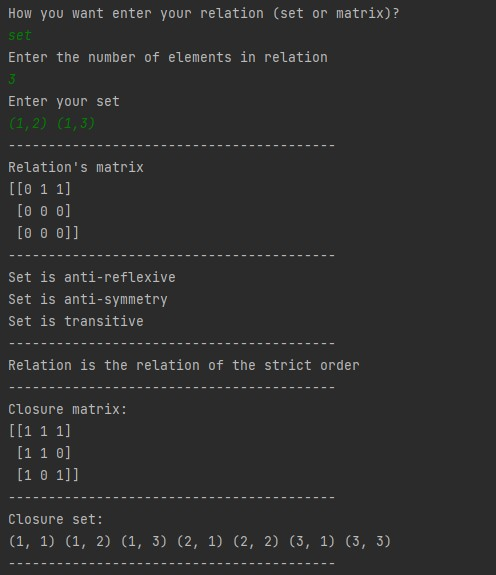
\includegraphics[width=1.\textwidth]{1}
            \caption{Тест алгоритма построения фактор множества}
            \label{fig:image1}
        \end{figure}
        
        \begin{figure}[H]
            \centering      %размер рисунка       здесь находится название файла рисунка, без указания формата
            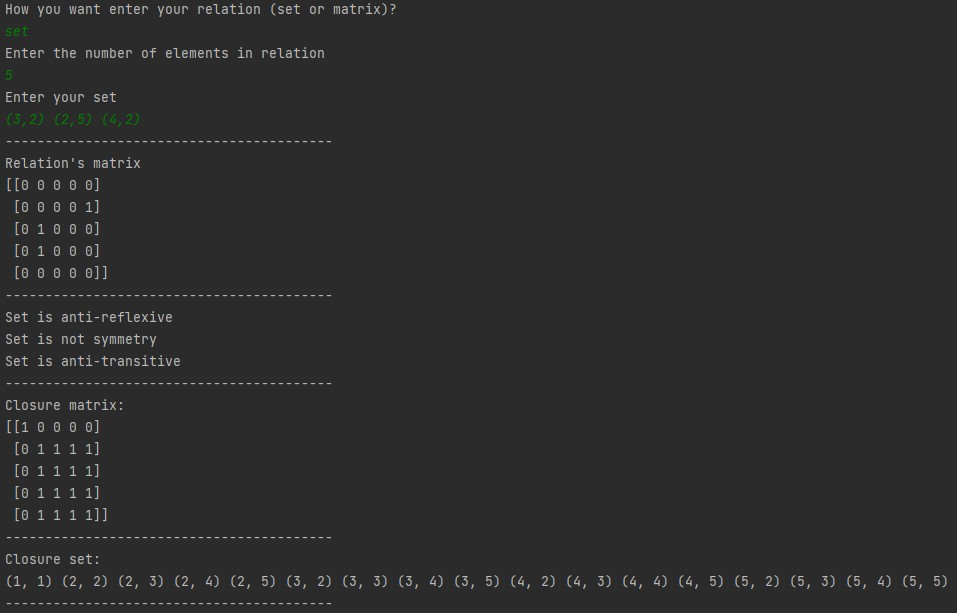
\includegraphics[width=1.\textwidth]{2}
            \caption{Тест алгоритма построения диаграммы Хассе и поиска максимального(минимального) и наибольшего(наименьшего) элемента множества}
            \label{fig:image1}
        \end{figure}

        \begin{figure}[H]
            \centering      %размер рисунка       здесь находится название файла рисунка, без указания формата
            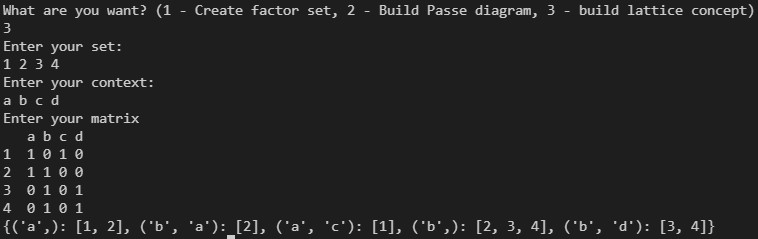
\includegraphics[width=1.\textwidth]{3}
            \caption{Тест алгоритма построения решетки концептов}
            \label{fig:image1}
        \end{figure}

        \subsection{Оценки сложности рассмотренных алгоритмов}

        \subsubsection{Алгоритм построения эквивалентного замыкания бинарного отношения}

        С учетом результатов вычисления асимптотики для первой лабораторной работы, алгоритм эквивалентного замыкания имеет асимптотику $O(n^4)$.

        \subsubsection{Алгоритм системы представителей.}
            С учетом наличия одного вложенного цикла и применения быстрой сортировки, алгоритм системы представителей имеет асимптотику $O(n^2 + nlogn) = O(n^2)$.
        \subsubsection{Алгоритм нахождения минимальных (максимальных) элементов множества.}
            Временная сложность получения срезов составляет $O(n^2)$, сложность нахождение минимальных (максимальных) элементов по длине
            среза составляет $O(n)$. Исходя из всего этого временная сложность алгоритма составляет $O(n^2)$.
        \subsubsection{Алгоритм нахождения наименьших (наибольших) элементов множества.}
            Если не учитывать асимптотику алгоритма нахождения минимальных (максимальных) элементов множества, который используется
            в этом алгоритме, то сложность составляет $O(1)$, с учетом вышеописанного алгоритма асимптотика определяется как
            $O(n^2)$.
        \subsubsection{Алгоритм построения диаграммы Хассе.}
            С учетом наличия двух вложенных циклов, алгоритм построения диаграммы Хассе имеет асимптотику $O(n^3)$.

        \subsubsection{Алгоритм построения решетки концепта.}
            Асимптотика получения среза по столбцу атрибутов составляет $O(n^2)$, а эти срезы мы получаем $k^2$ раз. 
            Следовательно алгоритм построения решетки концептов имеет асимптотику $O(k^2 \cdot n^3)$.
\conclusion

В рамках данной лабораторной работы были рассмотренны теоритические основы  отношений эквивалентности, построение их фактор
множеств, построение диаграмм Хассе и решетки концептов. На основе этой теоретической части была смоделирована программа на языке Python с 
использованием средств библиотеки Numpy, которая способна пострить замыкание эквивалентности, фактор множество, систему представителей этого множества,
построить диаграмму Хассе на отношение делимости и построить решетку концептов для заданного множества, а так же была оценена асимптотика каждого реализованного
алгоритма.

\end{document}
